\chapter{粒子力学から古典場へ}

\section{場とは何か}

前回の講義では、不変な作用から相対論的粒子力学を展開した。ここで力学変数を変更する。主題は古典場の理論であり、量子場の理論ではない。量子力学は時に有用な比較を与えるが、本章の方程式が記述するのは通常の古典場である。電磁気学は背景にある馴染み深いモデルである。電磁波は空間を伝播し、荷電粒子と相互作用する。まずはさらに単純な場から始める。

時空は多くの空間座標を持ちうるが、時間座標は一つである。
\begin{equation}
x^\mu=(t,x^1,\ldots,x^d),
\end{equation}
と書く。ここで空間添字は\(i=1,\ldots,d\)である。数\(d\)は、我々の世界のように3であってもよいし、1、2、9、25、あるいはモデルに有用なその他の任意の数であってもよい。この段階で重要な非対称性は、依然として時間方向が一つしかないことである。本講義は、複数の時間を持つ理論がなぜそれほど困難であるかを説明しようとはせず、通常の因果的な物理学が定式化される一時間の枠組みを単に採用する。

場とは、点から点へ、また時から時へと値が変化しうる可測量である。温度は単純な例である。
\begin{equation}
T=T(\mathbf{x},t).
\end{equation}
これは各事象に一つの数を割り当てるので、スカラー場である。風速も空間と時間にわたって変化するが、大きさと向きを持ち、したがって複数の成分を持つ。これはベクトル場である。相対論的物理学では、自然なベクトルは3成分ではなく4成分を持つ。

本講義の大部分では、場は一つの成分を持ち、\(f\)に対応するギリシア文字で表される。
\begin{equation}
\phi=\phi(\mathbf{x},t).
\label{eq:sr4-field-definition}
\end{equation}
\(\phi\)をスカラーと呼ぶことは、やがてそれが一つの成分を持つという以上の意味を持つようになる。それは、すべての慣性観測者が同じ物理的事象において\(\phi\)に同じ値を割り当てることを意味する。その変換則は、変分力学が構築された後に初めて登場する。

\section{粒子の原型}

\subsection{\texorpdfstring{\(\phi\)}{phi}という座標}

場の理論への最短の道は、通常の非相対論的粒子に立ち返ることから始まる。粒子を直線上で運動させるが、その座標を\(x\)ではなく\(\phi\)と呼ぶ。座標を\(x\)と名付ける数学的な義務はない。この珍しい名前は、これから来る類推を可視化するために選ばれている。時間を水平に描く。すると粒子の全履歴は曲線\(\phi(t)\)となり、正の値と負の値を通過しうる。

固定された初期時刻と最終時刻\(a\)および\(b\)に対して、作用は
\begin{align}
A[\phi]
&=\int_a^b dt\,L(\phi,\dot\phi),\\
L(\phi,\dot\phi)
&=\frac{m}{2}\dot\phi^{\,2}-V(\phi).
\label{eq:sr4-particle-lagrangian}
\end{align}
である。Euler--Lagrange方程式は
\begin{equation}
\frac{d}{dt}\left(\frac{\partial L}{\partial\dot\phi}\right)
-\frac{\partial L}{\partial\phi}=0.
\label{eq:sr4-particle-el}
\end{equation}
である。\eqref{eq:sr4-particle-lagrangian}のLagrangianに対して、
\begin{equation}
\frac{\partial L}{\partial\dot\phi}=m\dot\phi,
\qquad
\frac{\partial L}{\partial\phi}=-\frac{dV}{d\phi},
\end{equation}
であるから、
\begin{equation}
\boxed{m\ddot\phi=-\frac{dV}{d\phi}}.
\label{eq:sr4-newton}
\end{equation}
となる。これは単に、\(\phi\)を座標として書かれたNewtonの方程式である。

\begin{figure}[htbp]
\centering
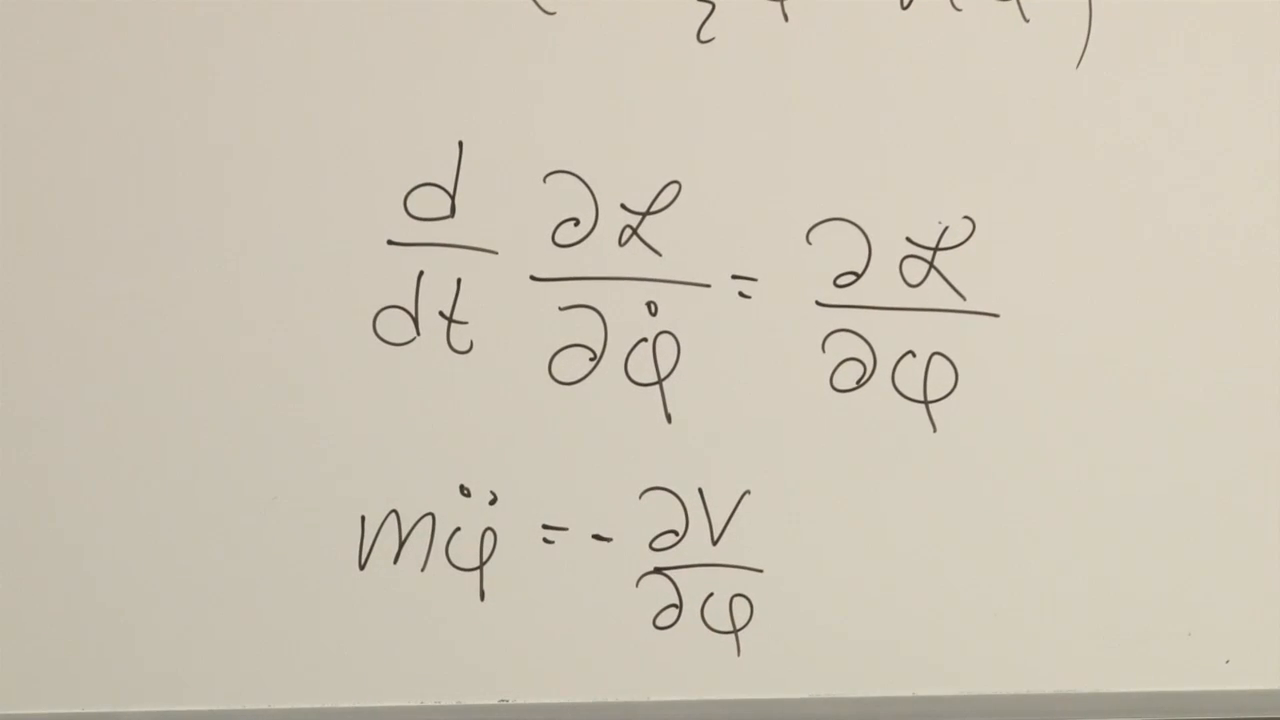
\includegraphics[width=0.90\textwidth]{lecture_04_figure_01.png}
\caption{通常のEuler--Lagrange方程式と、座標\(\phi(t)\)に対するそのNewton的な結果。}
\lectureframe{00:10:18}
\end{figure}

物理的な経路は、端点を固定したまま作用を停留させる。本講義ではしばしば\emph{最小}と言うが、正確な記述は停留性である。経路は最小値を与えることも、最大値を与えることも、あるいは別の停留値を与えることもある。有用な心的モデルの一つは、時間区間を多くの小さな断片に分割することである。作用は、\(\phi\)の多くのサンプル値の関数となる。端点を固定したままそれらの値を動かし、それぞれについて微分することは、Euler--Lagrange方程式の有限次元の祖先である。

\subsection{\texorpdfstring{\(0+1\)}{0+1}次元における理論としての力学}

ここで、時間はあるが空間次元がない世界を想像しよう。その空間は単一の点である。その世界の場は位置に依存しえない。依存すべき位置が存在しないからである。それは関数\(\phi(t)\)にしかなりえない。したがって、通常の一座標の粒子力学は、\(0+1\)次元における場の理論として読むことができる。数学は変わっていない。変わるのは、粒子の位置から、空間のない世界における場の値へという解釈だけである。

\begin{figure}[htbp]
\centering
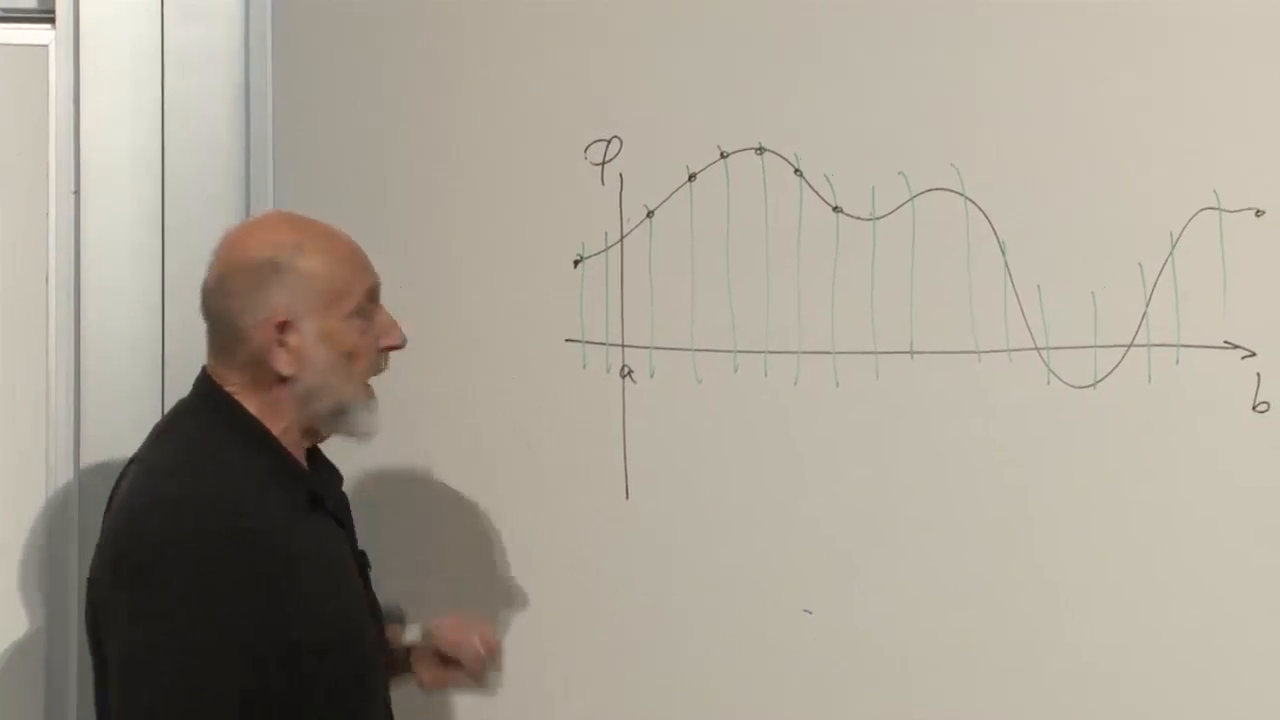
\includegraphics[width=0.90\textwidth]{lecture_04_figure_02.png}
\caption{サンプルされた履歴\(\phi(t)\)：粒子の軌道、そして新しい解釈のもとでは、\(0+1\)次元における場の履歴。}
\lectureframe{00:14:30}
\end{figure}

\begin{classroomqa}
\audiencequestion{空間次元が存在しないとき、ポテンシャルは消えるのか。}
\lecturerresponse{消えない。空間的な変化は消えるが、場は依然として値をもつ。エネルギーは\(V(\phi)\)を通じてその値に依存しうる。粒子解釈では、曲線を上下に動かすとポテンシャルエネルギーが変わる。場の解釈では、\(\phi\)の異なる値が異なるポテンシャルエネルギーを担う。\lecturetimestamp{00:15:00}}
\end{classroomqa}

\begin{classroomqa}
\audiencequestion{空間がまったくないと想像する代わりに、場が時間のみに依存する通常の空間を想像してもよいか。}
\lecturerresponse{よい。この目的には局所的な数学は同じである。すべての空間微分が消え、\(\phi(t)\)だけが残る。これを\(0+1\)次元理論と呼ぶとその縮約された構造が切り出されるが、より大きな世界における空間的に一様な場も同じ直観を与える。\lecturetimestamp{00:16:25}}
\end{classroomqa}

この回り道の要点は今や明らかである。われわれは、一つの座標、すなわち時間のみに依存する場に対する作用原理を知っている。そのパターンを用いて、時空のすべての座標に依存する場に対する作用原理を推測できる。

\section{時空上の場の歴史}

\subsection{曲線から曲面へ}

\(1+1\)次元では、時空自体が座標\(t\)と\(x\)をもつ平面である。値\(\phi(x,t)\)が第三の方向を与える。したがって場の歴史は曲線ではなく、時空平面の上の曲面である。スカラー場は正である必要はないので、曲面はゼロより上に隆起しても下に沈んでもよい。

\begin{figure}[htbp]
\centering
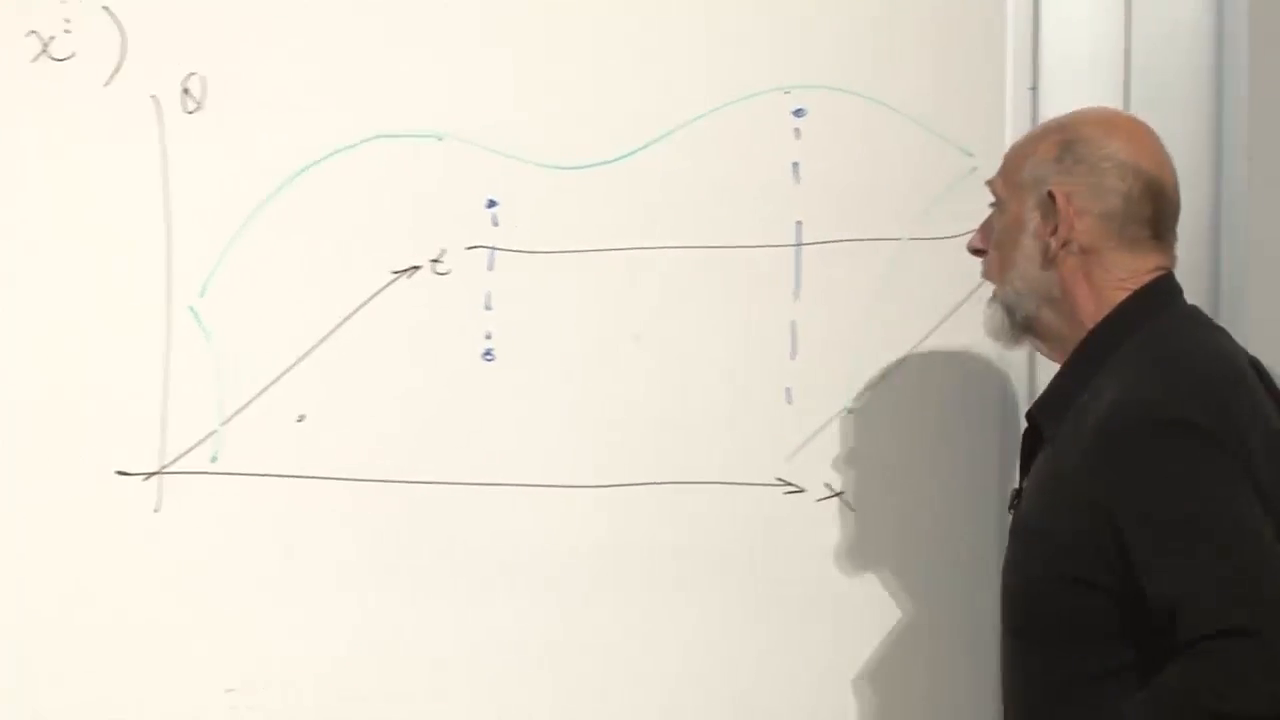
\includegraphics[width=0.90\textwidth]{lecture_04_figure_03.png}
\caption{\(1+1\)次元時空平面上の曲面として描かれたスカラー場の歴史。}
\lectureframe{00:20:46}
\end{figure}

われわれの物理的時空は\(3+1\)次元と呼ばれる。すなわち3つの空間次元と1つの時間次元である。卓上の模型は\(2+1\)次元であり、針金に拘束されたビーズは\(1+1\)次元世界を示唆する。\(\phi\)をプロットするために必要な余分な軸のため、\(3+1\)の場合でさえ忠実に描くことは不可能であるが、定義は曖昧でない。完全な歴史は、すべての時空事象に\(\phi\)の一つの値を割り当てる。

\subsection{固定された端点から固定された境界データへ}

粒子の変分問題は2つの端点を固定し、その間の曲線を変化させる。その場の理論における類似は、時空領域を選び、その領域の境界上で\(\phi\)を固定し、内部で\(\phi\)を変化させる。領域は\(1+1\)次元の図における長方形でも、より高次元の時空における任意の適切な領域でもよい。

\begin{figure}[htbp]
\centering
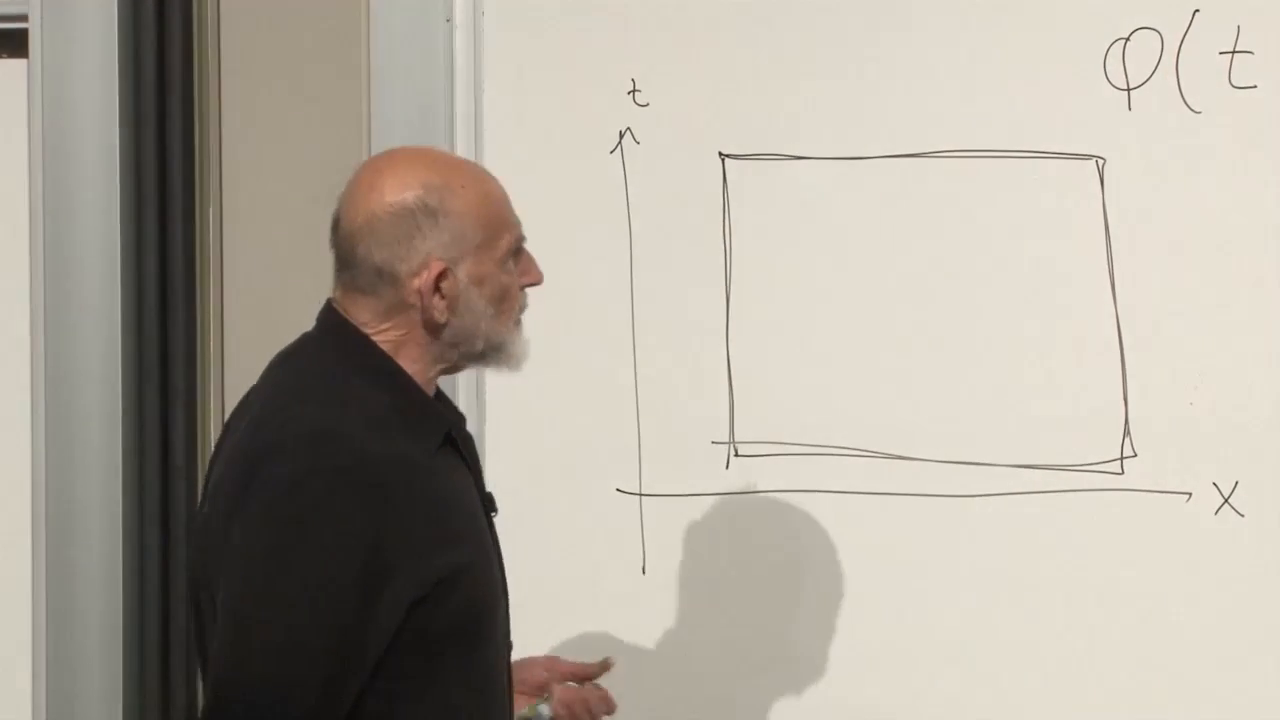
\includegraphics[width=0.90\textwidth]{lecture_04_figure_04.png}
\caption{境界全体が固定され、内部の場が変化させられる時空領域。}
\lectureframe{00:24:52}
\end{figure}

\begin{classroomqa}
\audiencequestion{ポテンシャルが時間に陽に依存するときでも、ラグランジアン形式は依然として機能するか。}
\lecturerresponse{機能する。オイラー--ラグランジュ形式およびハミルトン形式は依然として機能する。一般に失われるのはエネルギー保存である。時間への陽な依存は時間並進対称性を破る。場の理論における対応する主張は、時空への陽な依存は許されるが、それは関連する保存則に影響するというものである。\lecturetimestamp{00:23:49}}
\end{classroomqa}

\begin{classroomqa}
\audiencequestion{長方形の場の領域について、固定されるのは上下のみか、それとも境界全体か。}
\lecturerresponse{この変分構成では、境界全体が固定される。\(1+1\)次元の長方形における4つの辺すべてである。場は内部でのみ揺らぐことが許される。これは粒子力学において両端点を固定することの直接の類似である。\lecturetimestamp{00:24:24}}
\end{classroomqa}

境界全体を固定することは、方程式を導出するために用いられる変分についての主張である。得られた双曲型場の方程式を物理的な発展問題として扱うときには、適切な初期データを指定し、方程式にそれを前方へ伝播させることのほうがより一般的であろう。

\section{作用と場のオイラー--ラグランジュ方程式}

\subsection{ラグランジアン密度}

時空領域を小さなセルに分割する。作用は局所的な寄与の和、すなわち各セルからの寄与の和であると仮定される。連続極限ではその和は時空上の積分になる。
\begin{equation}
A[\phi]
=
\int_{\Omega} d^4x\,
\mathcal{L}\!\left(
\phi,\partial_\mu\phi;x^\mu
\right),
\qquad
d^4x=dt\,dx\,dy\,dz.
\label{eq:sr4-field-action}
\end{equation}
量\(\mathcal{L}\)はラグランジアン密度である。\(\mathcal{L}(\phi,\partial_\mu\phi;x^\mu)\)におけるセミコロンは、力学的な引数を可能な陽な座標依存から分離する。一様な閉じた系ではその最後の依存は通常存在しないが、変分形式はそれを禁じない。

簡潔な記法
\begin{equation}
\partial_\mu\phi
\equiv
\frac{\partial\phi}{\partial x^\mu}
\end{equation}
は時間微分と空間微分をまとめたものである。講義の成分表記では、代わりに
\begin{equation}
\begin{aligned}
\phi_t&=\frac{\partial\phi}{\partial t},\\
\phi_x&=\frac{\partial\phi}{\partial x},\\
\phi_y&=\frac{\partial\phi}{\partial y},\\
\phi_z&=\frac{\partial\phi}{\partial z}.
\end{aligned}
\label{eq:sr4-component-derivatives}
\end{equation}
と書いてもよい。粒子が複数の座標をもちうるように、場も複数ありうる。今のところ場は\(\phi\)ただ一つである。

記号\(d^4x\)は四次元座標の測度を表す略記にすぎない。別の次元の時空では、それは\(d^Dx\)に置き換えられる。\(0+1\)次元の原型では、\(D=1\)であり、\(d^1x\)は単に\(dt\)である。

\begin{figure}[htbp]
\centering
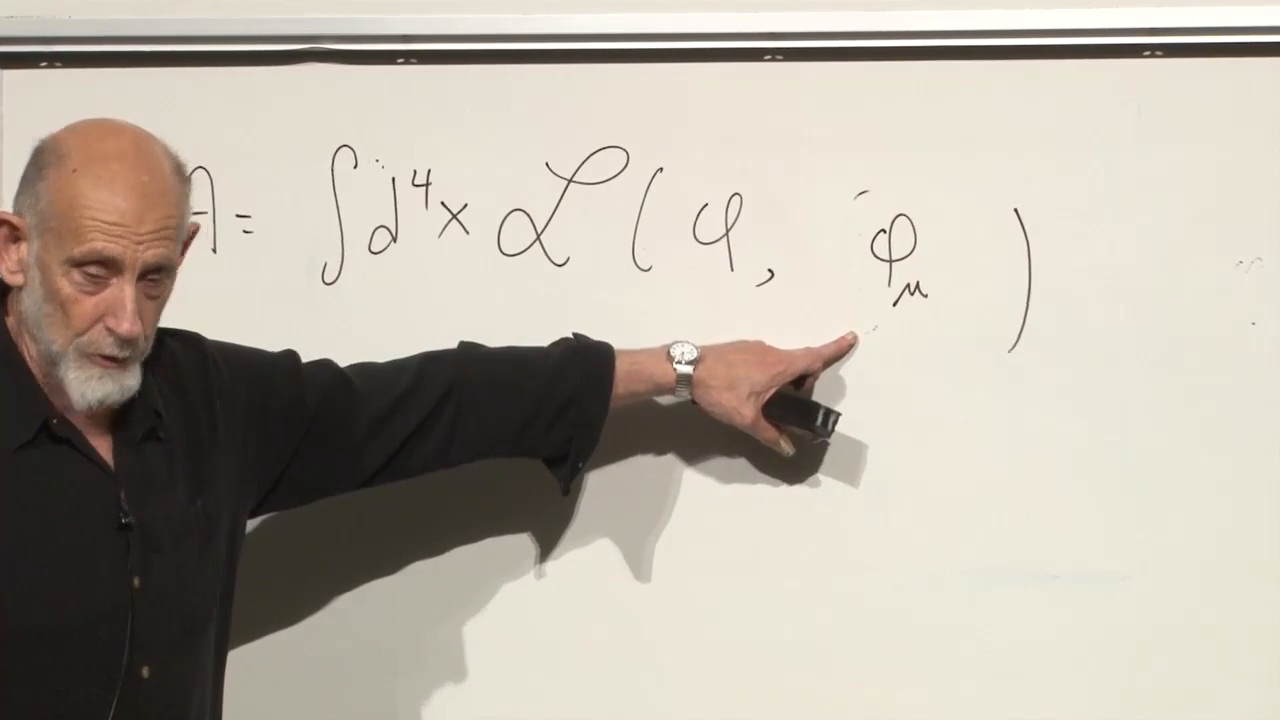
\includegraphics[width=0.90\textwidth]{lecture_04_figure_05.png}
\caption{\(\phi\)とその時空微分の局所関数として書かれた作用密度。}
\lectureframe{00:32:51}
\end{figure}

\begin{classroomqa}
\audiencequestion{ラグランジアン密度は\(x,y,z\)自身にも依存しうるか。}
\lecturerresponse{依存しうる。ちょうど粒子のラグランジアンが\(t\)に陽に依存しうるのと同じである。並進不変な閉じた系では通常は依存しないが、座標への陽な依存があっても形式論が無効になるわけではない。\lecturetimestamp{00:30:29}}
\end{classroomqa}

\begin{classroomqa}
\audiencequestion{これまでの構成はスカラー場に固有のものか、それとも一般的なものか。}
\lecturerresponse{これまでのところ変分のパターンは一般的である。成分を一つだけ書くとスカラー場を示唆する。ベクトル場や場の集まりならば追加の成分ラベルをもち、すべての成分を変分することになる。\lecturetimestamp{00:31:00}}
\end{classroomqa}

\subsection{格子の描像}

細かい時空格子上では、微分は隣り合う場の値の間の有限差分になる。すると作用は多数変数の通常の関数となる。一方向に十点、別の方向に八点をもつ格子でも、すでに八十個の場の変数を与える。格子を細かくすればその数は増えるが、最小化の規則は初等的なままであう。各内部点における場の値について作用を微分し、その結果をゼロと置くのである。

\begin{figure}[htbp]
\centering
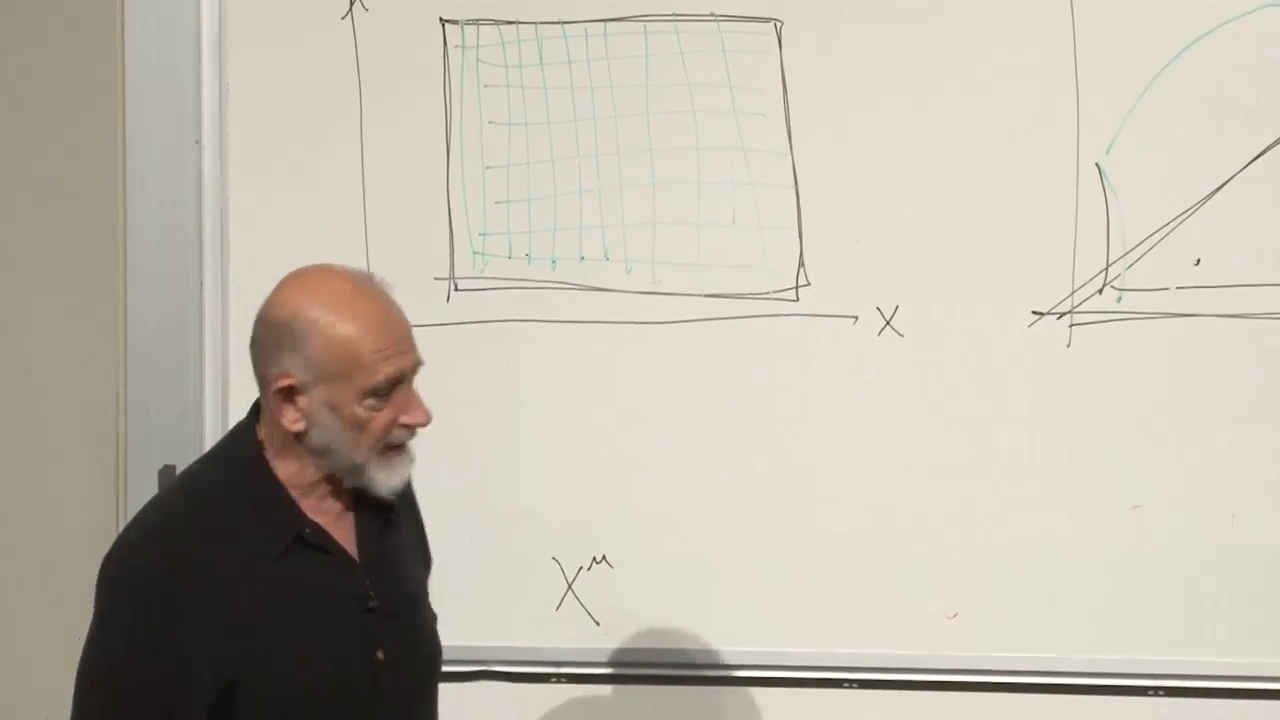
\includegraphics[width=0.90\textwidth]{lecture_04_figure_06.png}
\caption{時空領域をセルに分割し、連続極限の前に作用を通常の多変数関数とする。}
\lectureframe{00:34:05}
\end{figure}

連続極限を取ると場のオイラー--ラグランジュ方程式が得られる。
\begin{equation}
\boxed{
\partial_\mu
\left[
\frac{\partial\mathcal{L}}
{\partial(\partial_\mu\phi)}
\right]
-
\frac{\partial\mathcal{L}}{\partial\phi}
=0
}.
\label{eq:sr4-field-el}
\end{equation}
繰り返された\(\mu\)はすべての時空方向にわたって和を取る。和の略記を用いずに書けば、同じ方程式は
\begin{align}
&
\frac{\partial}{\partial t}
\left(\frac{\partial\mathcal{L}}{\partial\phi_t}\right)
+
\frac{\partial}{\partial x}
\left(\frac{\partial\mathcal{L}}{\partial\phi_x}\right)
+
\frac{\partial}{\partial y}
\left(\frac{\partial\mathcal{L}}{\partial\phi_y}\right)
\nonumber\\
&\hspace{3em}
+
\frac{\partial}{\partial z}
\left(\frac{\partial\mathcal{L}}{\partial\phi_z}\right)
-
\frac{\partial\mathcal{L}}{\partial\phi}
=0.
\label{eq:sr4-field-el-expanded}
\end{align}
となる。第一項はおなじみの粒子の項である。場の理論では各空間方向に対して同様の項が加わる。最後の項
\(-\partial\mathcal{L}/\partial\phi\)は変わらない。

\begin{figure}[htbp]
\centering
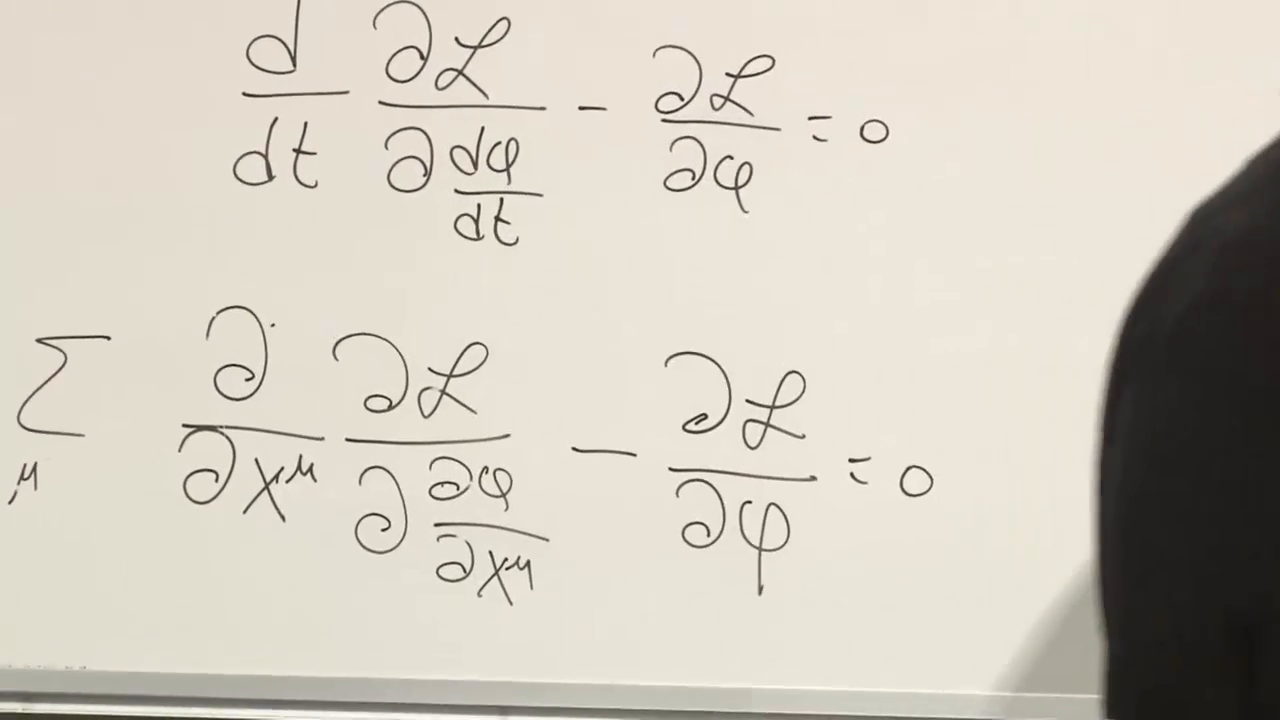
\includegraphics[width=0.90\textwidth]{lecture_04_figure_07.png}
\caption{一次元のオイラー--ラグランジュ方程式とその時空への一般化を上下に並べて書いたもの。}
\lectureframe{00:38:44}
\end{figure}

この主題は連続体力学とも呼ばれる。自由度に応じて、同じ数学が流体の流れ、弾性変位、あるいは別の連続媒質を記述しうる。

\begin{classroomqa}
\audiencequestion{空間はあるが時間のない世界でも同じ方程式は成り立つか。}
\lecturerresponse{成り立つ。純粋に空間的な変分問題としてである。物理的には、これが静的解を探す方法である。場が時間に依存しないと仮定し、すべての時間微分を捨て、残った空間的方程式を解く。時間に依存しない電気的あるいは磁気的配置がその例である。\lecturetimestamp{00:40:05}}
\end{classroomqa}

\section{最も単純なスカラー力学を推測する}

\subsection{なぜ符号がすべて一致しえないのか}

粒子の運動項\(\tfrac12\dot\phi^2\)に戻り、無関係な全体の係数を一に置いて、それを一般化しようと試みる。最初の推測は
\begin{equation}
\mathcal{L}_{+}
=
\frac12
\left[
\phi_t^2+\phi_x^2+\phi_y^2+\phi_z^2
\right].
\label{eq:sr4-all-plus}
\end{equation}
かもしれない。これは有益な誤りである。時間と空間を同一の符号で扱っている。得られる方程式は波動伝播の双曲的構造をもたないであろう。正しい相対論的組み合わせでは、時間に一つの符号、空間に反対の符号がつく。

\begin{classroomqa}
\audiencequestion{すべてプラスの表式が誤りであるのは、ラグランジアンが相対論的に不変であるべきだからか。}
\lecturerresponse{それがより深い答えであり、正しい。講義ではまずより素朴に符号に到達する。波は時間における発展と空間における変動を区別するので、時間は別の空間座標とまったく同じようには入りえない。ローレンツ不変性がまもなくその直観を精密な規則に変える。\lecturetimestamp{00:43:19}}
\end{classroomqa}

特徴的な速さ\(c\)を復元すると、単純なスカラーラグランジアン密度は
\begin{equation}
\boxed{
\mathcal{L}
=
\frac12
\left[
\frac{1}{c^2}\phi_t^2
-\phi_x^2-\phi_y^2-\phi_z^2
\right]
-V(\phi)
}.
\label{eq:sr4-scalar-lagrangian}
\end{equation}
となる。相対論的な場では、\(c\)は光速である。連続体模型では、代わりに音速、弾性波の速さ、あるいは別の特徴的な伝播速度でありうる。

全体の因子 \(1/2\) は、\(\tfrac12m\dot\phi^2\) における場合と同様に慣習的なものである。作用全体にゼロでない定数を掛けてもその停留経路は変わらない。この慣習は、方程式中のパラメータがどのように名付けられ、規格化されるかを定める。ひとたびその規格化を選んだならば、一貫してそれを使わなければならない。

\begin{classroomqa}
\audiencequestion{空間勾配の項をポテンシャルエネルギーの一部と見なせるか。}
\lecturerresponse{はい。運動エネルギーからポテンシャルを引くという構成では、運動エネルギー部分は時間微分を含む。時間微分を含まない項、すなわち空間勾配や \(V(\phi)\) は、ポテンシャルエネルギー側に属する。相対論的理論においてそれらの相対的な符号がそうなる究極の理由は、ローレンツ計量である。\lecturetimestamp{00:45:37}}
\end{classroomqa}

\subsection{波動方程式}

\eqref{eq:sr4-field-el} を適用する。微分の項は
\begin{equation}
\frac{\partial\mathcal{L}}{\partial\phi_t}
=\frac{1}{c^2}\phi_t,
\qquad
\frac{\partial\mathcal{L}}{\partial\phi_i}
=-\phi_i,
\end{equation}
であり、一方
\begin{equation}
\frac{\partial\mathcal{L}}{\partial\phi}
=-\frac{dV}{d\phi}.
\end{equation}
である。したがって
\begin{equation}
\begin{aligned}
&\boxed{
\frac{1}{c^2}\frac{\partial^2\phi}{\partial t^2}
-\nabla^2\phi
+\frac{dV}{d\phi}
=0
},\\[0.5em]
\nabla^2
&=
\frac{\partial^2}{\partial x^2}
+\frac{\partial^2}{\partial y^2}\\
&\quad
+\frac{\partial^2}{\partial z^2}.
\end{aligned}
\label{eq:sr4-general-scalar-eom}
\end{equation}

\(V=0\) ならば、これは
\begin{equation}
\boxed{
\frac{1}{c^2}\phi_{tt}-\nabla^2\phi=0
},
\label{eq:sr4-wave-equation}
\end{equation}
すなわち波動方程式に帰着する。講義はこの方程式を認識するが、その求解は後回しにする。その解は摂動を速さ \(c\) で伝播させる。

\begin{figure}[htbp]
\centering
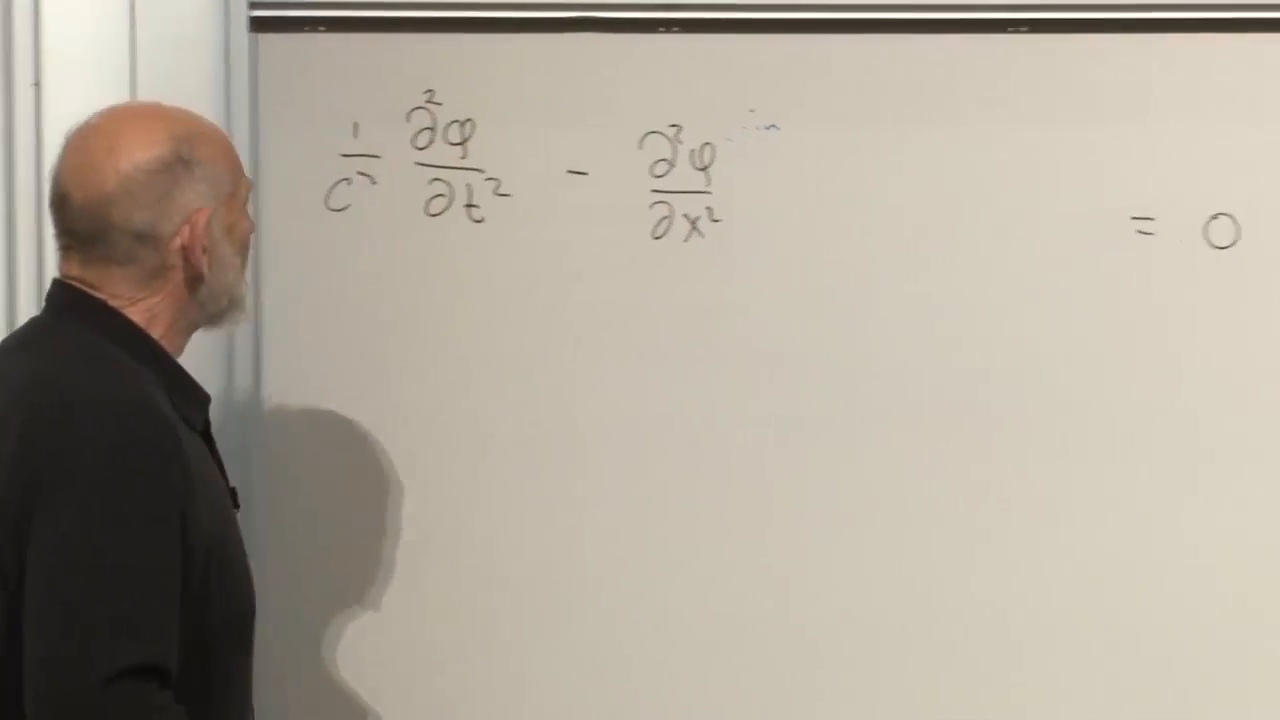
\includegraphics[width=0.90\textwidth]{lecture_04_figure_08.png}
\caption{一次元の形 \(c^{-2}\phi_{tt}-\phi_{xx}=0\) は、波動方程式として認識される。}
\lectureframe{00:50:30}
\end{figure}

\subsection{結合した調和振動子の場}

ここで二次のポテンシャルを選ぶ。
\begin{equation}
V(\phi)=\frac12\mu^2\phi^2,
\qquad
\frac{dV}{d\phi}=\mu^2\phi.
\label{eq:sr4-quadratic-potential}
\end{equation}
もし \(\phi\) が粒子の位置であれば、これはばね定数 \(\mu^2\) の調和振動子のポテンシャルであろう。場に対しては
\begin{equation}
\boxed{
\frac{1}{c^2}\phi_{tt}-\nabla^2\phi+\mu^2\phi=0
}.
\label{eq:sr4-klein-gordon}
\end{equation}
となる。空間微分がなければ、これは単に加速度に定数かける変位を加えたものがゼロに等しいという式である。勾配は隣接する点を結合し、振動子を波を担う連続体に変える。相対論的場の理論では \eqref{eq:sr4-klein-gordon} は質量をもつクライン--ゴルドン方程式と呼ばれる。古典的には、\(\mu\) は波の伝播を修飾する逆長さスケールである。

\begin{figure}[htbp]
\centering
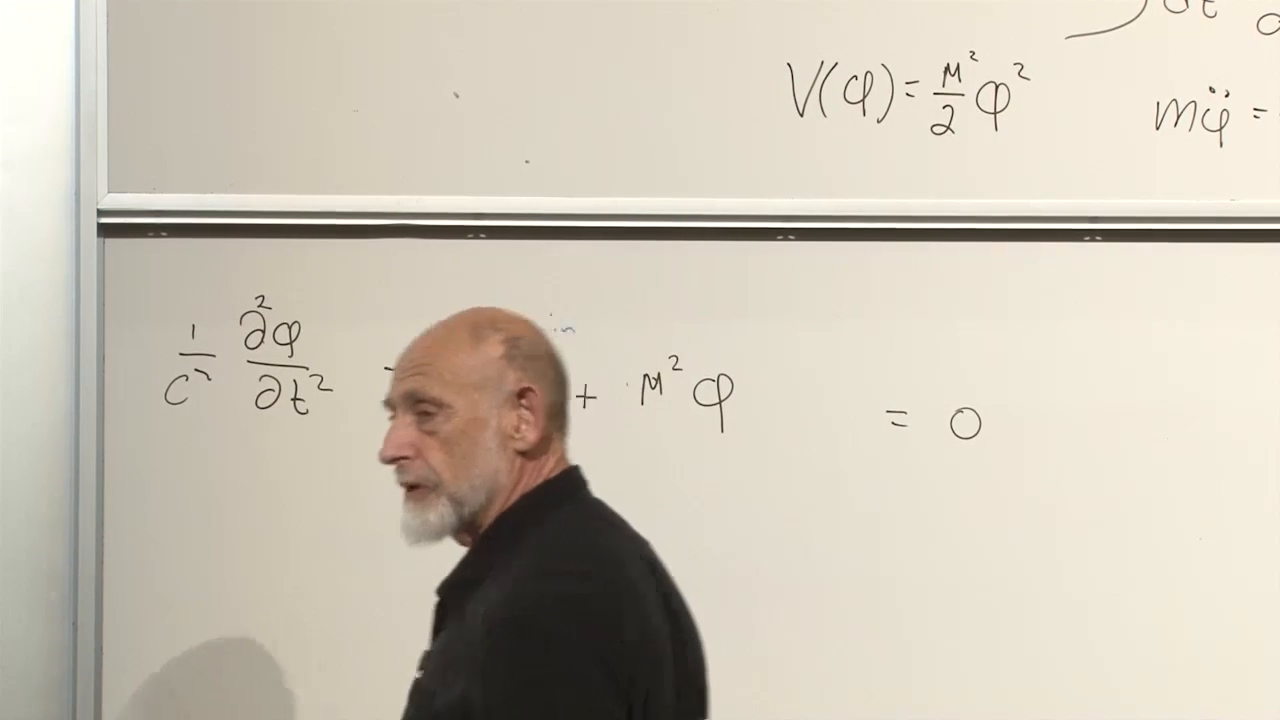
\includegraphics[width=0.90\textwidth]{lecture_04_figure_09.png}
\caption{二次のポテンシャルと、復元項 \(\mu^2\phi\) を伴う結果としての波動方程式。}
\lectureframe{00:52:38}
\end{figure}

\begin{classroomqa}
\audiencequestion{なぜ \(V=\tfrac12\mu^2\phi^2\) における因子 \(1/2\) は運動方程式から消えるのか。}
\lecturerresponse{\(\phi^2\) を微分すると因子 2 が現れる。慣習的な \(1/2\) は、ちょうど \(V(x)=\tfrac12kx^2\) が復元力 \(-kx\) を与えるのと同様に、\(dV/d\phi=\mu^2\phi\) となるようにまさに挿入されている。\lecturetimestamp{00:53:17}}
\end{classroomqa}

この方程式は線形である。\(\phi\) およびその各微分は一次でしか現れない。運動方程式における \(\phi^2\) や \(\phi\,\partial_\mu\phi\) のような項は、力学を非線形にするであろう。

\section{ローレンツスカラーと四元ベクトル}

\subsection{作用は座標系に依存してはならない}

変分の仕組みだけでも多くの可能な場の理論が定義される。相対性理論は、作用がすべての慣性系で同じ値と同じ形をもつという追加の要請を課す。自由粒子に対しては、これは世界線に沿って不変な固有時 \(d\tau\) を積分することによって達成された。場に対しては、作用は時空にわたって積分されるので、その局所的な構成要素は適切に変換しなければならない。

固有ローレンツ変換の下で時空の測度は不変である。\(d^4x'=d^4x\)。したがって、ラグランジアン密度がローレンツスカラーであることを要求すれば十分である。
\begin{equation}
\mathcal{L}'(x')=\mathcal{L}(x).
\label{eq:sr4-lagrangian-scalar}
\end{equation}

\subsection{スカラー場}

スカラー場は
\begin{equation}
\boxed{\phi'(x')=\phi(x)}.
\label{eq:sr4-scalar-transform}
\end{equation}
を満たす。座標 \(x\) と \(x'\) は二つの座標系において同じ事象をラベルする。観測者が用いる関数表現は異なって見えるかもしれないが、その物理的事象に付される数は同じである。

\begin{figure}[htbp]
\centering
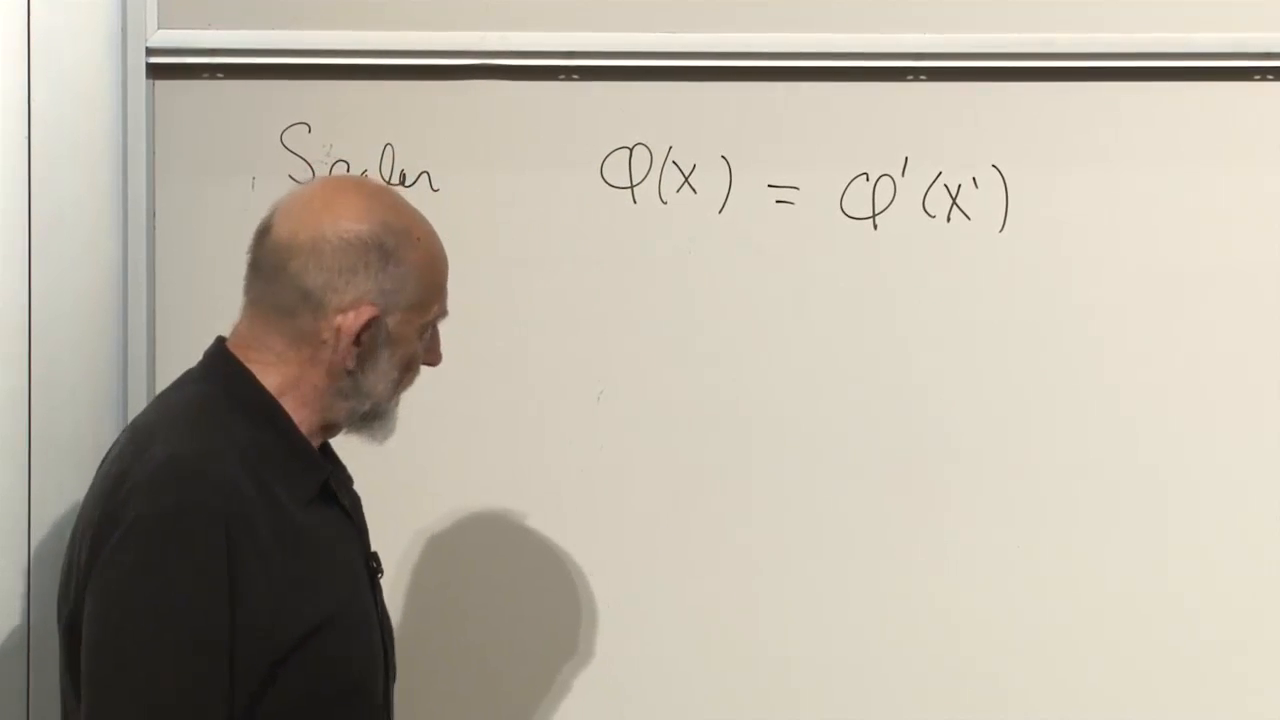
\includegraphics[width=0.90\textwidth]{lecture_04_figure_10.png}
\caption{スカラー場の定義的変換則: \(\phi(x)=\phi'(x')\)。}
\lectureframe{00:59:33}
\end{figure}

温度が初期の直観を与えたが、物質媒質中を動く温度計は完全な相対論的例ではない。温度計の類推よりも、定義 \eqref{eq:sr4-scalar-transform} こそが重要である。

\subsection{四元ベクトル}

単位 \(c=1\) では、\(x\) 軸に沿った速さ \(v\) のブーストは
\begin{equation}
\begin{aligned}
t'&=\gamma(t-vx),\\
x'&=\gamma(x-vt),\\
y'&=y,\\
z'&=z,\\
\gamma&=\frac{1}{\sqrt{1-v^2}}.
\end{aligned}
\label{eq:sr4-x-boost}
\end{equation}
として作用する。

\begin{figure}[htbp]
\centering
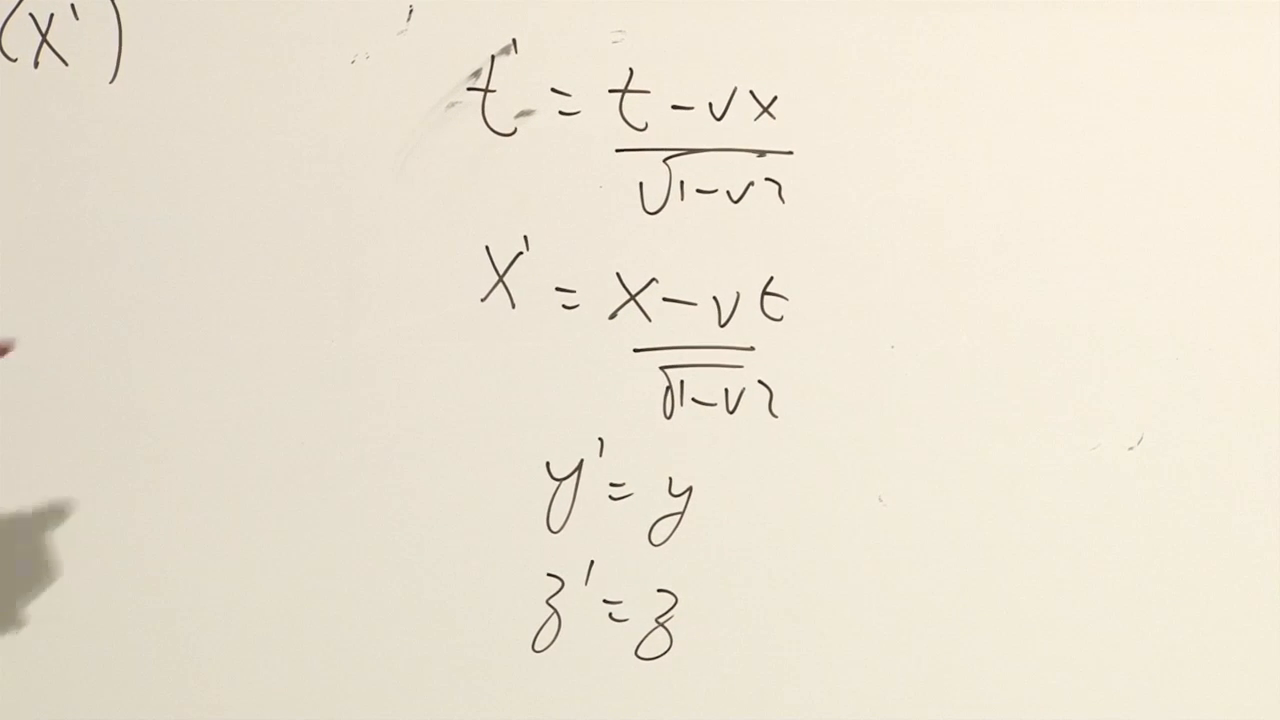
\includegraphics[width=0.90\textwidth]{lecture_04_figure_11.png}
\caption{\(c=1\) 単位における \(x\) 軸に沿ったブーストに対するローレンツ変換。}
\lectureframe{01:02:26}
\end{figure}

ブーストの下で同じように混ざり合う四つの量は四元ベクトルをなす。すでに現れた例は \(x^\mu\)、\(dx^\mu\)、および四元速度 \(u^\mu=dx^\mu/d\tau\) である。四元ベクトルにスカラーを掛けると別の四元ベクトルが得られる。流れる相対論的流体は場に値をもつ例を与える。その四元速度 \(u^\mu(x)\) は事象ごとに異なりうる。

\eqref{eq:sr4-x-boost} と同じブーストに対して、一般の四元ベクトルは
\begin{equation}
\begin{aligned}
A'^0&=\gamma(A^0-vA^x),\\
A'^x&=\gamma(A^x-vA^0),\\
A'^y&=A^y,\\
A'^z&=A^z.
\end{aligned}
\label{eq:sr4-vector-boost}
\end{equation}
を満たす。

一般の四元ベクトル \(A^\mu=(A^0,A^x,A^y,A^z)\) に対して、ローレンツ的ノルム
\begin{equation}
\boxed{
A_\mu A^\mu
=(A^0)^2-(A^x)^2-(A^y)^2-(A^z)^2
}
\label{eq:sr4-vector-norm}
\end{equation}
はスカラーである。これは、
\begin{equation}
d\tau^2=dt^2-dx^2-dy^2-dz^2
\end{equation}
が不変であるのと同じ代数的理由により不変である。講義では、一般のベクトルに使える未使用の文字が尽きかけ、矢印に対する \(A\) という提案に助けられて、最終的に \(A\) を受け入れる。

\begin{figure}[htbp]
\centering
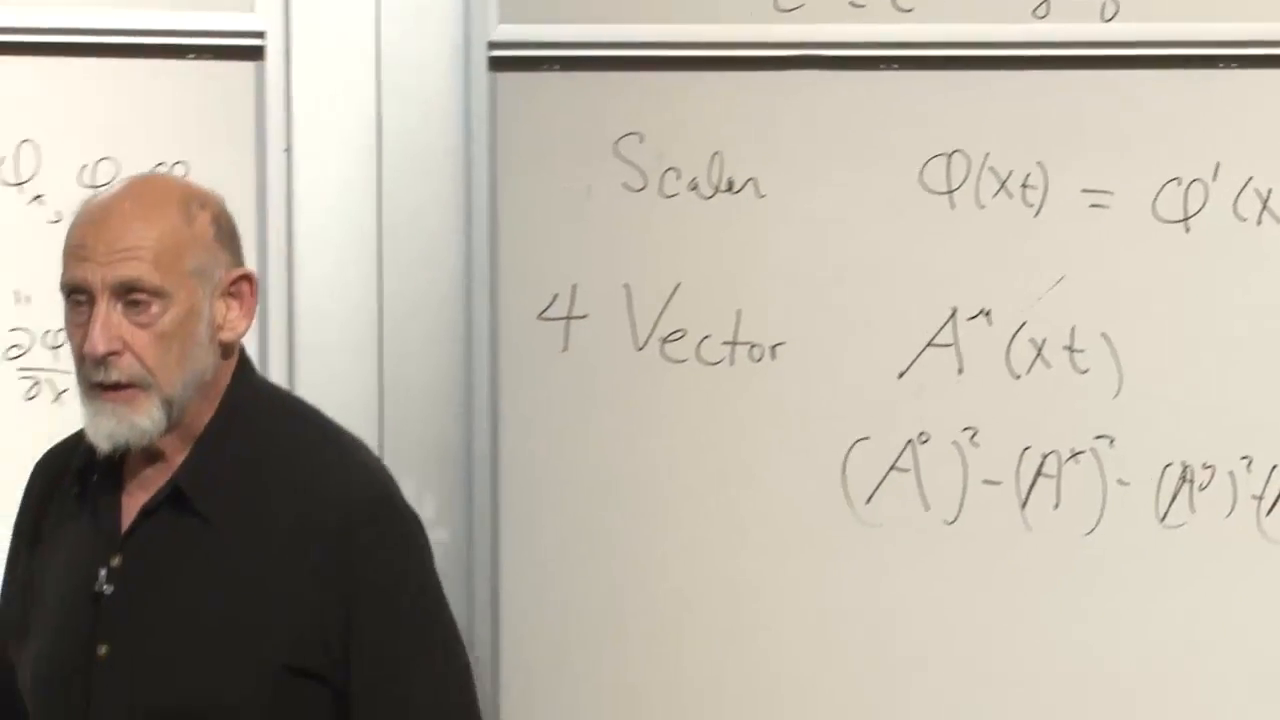
\includegraphics[width=0.90\textwidth]{lecture_04_figure_12.png}
\caption{一般の四元ベクトル場と、その不変ノルムを形成するローレンツ的二乗差。}
\lectureframe{01:09:06}
\end{figure}

\subsection{スカラーの微分}

スカラーを四つの時空座標で微分すると、四つの成分
\begin{equation}
\partial_\mu\phi
=
\left(
\frac{\partial\phi}{\partial t},
\frac{\partial\phi}{\partial x},
\frac{\partial\phi}{\partial y},
\frac{\partial\phi}{\partial z}
\right)
\qquad(c=1).
\end{equation}
が得られる。厳密には、\(\partial_\mu\phi\) は余ベクトルであり、ミンコフスキー計量がその添字を上げて \(\partial^\mu\phi\) にする。この区別はここでの成分による議論では無害であるが、縮約を曖昧さなく確定する：
\begin{equation}
\boxed{
\partial_\mu\phi\,\partial^\mu\phi
=
\frac{1}{c^2}\phi_t^2
-\phi_x^2-\phi_y^2-\phi_z^2
}.
\label{eq:sr4-derivative-scalar}
\end{equation}

\begin{figure}[htbp]
\centering
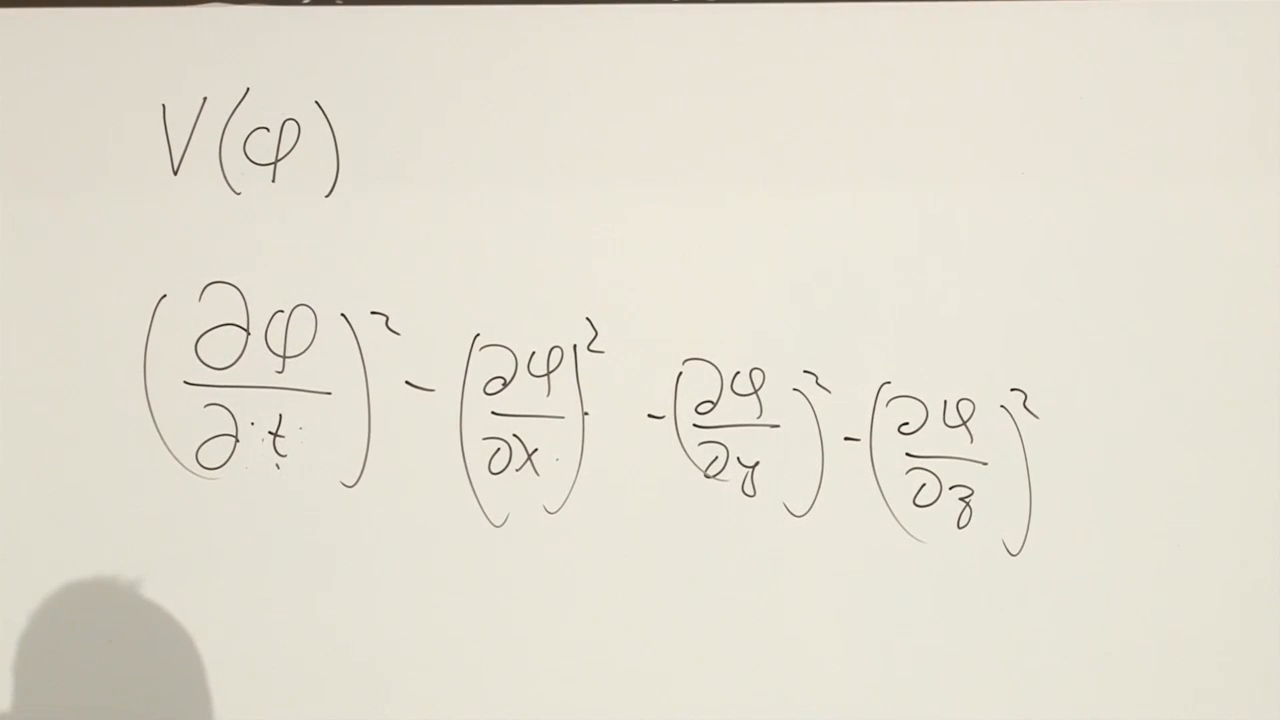
\includegraphics[width=0.90\textwidth]{lecture_04_figure_13.png}
\caption{スカラー場の一階微分から作られる不変な二乗差。}
\lectureframe{01:13:55}
\end{figure}

\begin{classroomqa}
\audiencequestion{この微分の組み合わせはラプラシアンか。}
\lecturerresponse{いいえ。表示された不変量は一階微分について二次である。ラプラシアンは二階の空間微分を含む。二階微分は作用を変分した後、波動方程式においてのみ現れる。\lecturetimestamp{01:13:22}}
\end{classroomqa}

\eqref{eq:sr4-scalar-lagrangian} の符号パターンは、今や推測ではなく説明される。運動項の勾配の組み合わせはローレンツスカラー
\(\partial_\mu\phi\,\partial^\mu\phi\)
である。したがって、最も単純な二次理論は
\begin{equation}
\mathcal{L}
=
\frac12\partial_\mu\phi\,\partial^\mu\phi
-\frac12\mu^2\phi^2.
\label{eq:sr4-covariant-lagrangian}
\end{equation}

\begin{figure}[htbp]
\centering
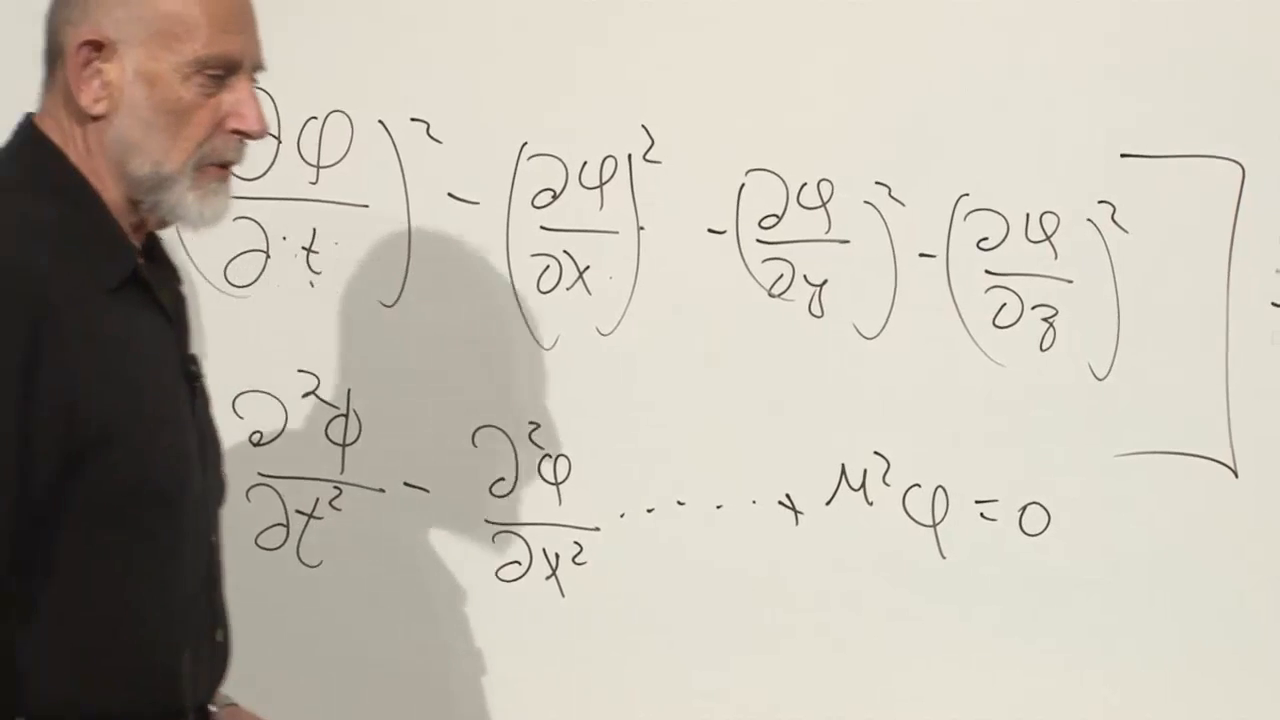
\includegraphics[width=0.90\textwidth]{lecture_04_figure_14.png}
\caption{完成した二次スカラー場ラグランジアンと、その線形場の方程式が黒板に示されている。}
\lectureframe{01:19:12}
\end{figure}

\section{どれほどの自由度があるか}

スカラーを構成する規則が分かれば、多くのラグランジアンが可能になる。場 \(\phi\) はスカラーであるから、任意の通常の関数 \(F(\phi)\) もまたスカラーである：\(\phi^2\)、\(\phi^3\)、\(\cosh\phi\) など。数値パラメータも許される。\(\mu\) のような記号を定数係数として挿入してもよい。残る問題はその次元と物理的解釈だけである。

\begin{classroomqa}
\audiencequestion{ラグランジアンに質量を入れることができるか。}
\lecturerresponse{定数パラメータなら確かに入れられる。この段階では、それがどの対象の質量なのかを問うべきである。なぜなら、\(\mu\) はその物理的意味が同定されるまでは古典場の理論における単なる数だからである。二次の相対論的スカラー理論では、それは質量または逆長さのスケールを定める。\lecturetimestamp{01:14:16}}
\end{classroomqa}

スカラーは掛け合わせてもよい：
\begin{equation}
F(\phi)\,\partial_\mu\phi\,\partial^\mu\phi
\end{equation}
はローレンツ不変である。微分スカラーそれ自体を二乗し、一階微分のより高次の冪を作ることもできる。より高次の微分を考えることもできるが、講義では場とその一階微分に注意を限定する。これは二階の運動方程式を与える標準的な枠組みである。高階微分理論は、一般に余分な力学的情報と起こりうる不安定性を導入するため、追加の注意を要する。

\begin{classroomqa}
\audiencequestion{二乗差の構成は本当に時空の計量なのか。}
\lecturerresponse{はい。選んだ符号規約では計量は \(dt^2-dx^2-dy^2-dz^2\) である。講義ではまだ計量という語を強調していないが、これはまさに一般相対性理論で中心となる時空幾何である。\lecturetimestamp{01:19:39}}
\end{classroomqa}

\begin{classroomqa}
\audiencequestion{\(xy\) や \(tx\) のような成分をもつ、四元ベクトルより一般的な対象はあるか。}
\lecturerresponse{はい。それらはテンソルである。スカラーは時空添字をもたず、ベクトルは一つもち、二階テンソルは \(T^{xx}\)、\(T^{xy}\)、\(T^{tx}\) のような成分をもつ。現在のスカラー場の議論の大部分はそれらを避けているが、一般相対性理論では避けられなくなる。\lecturetimestamp{01:20:49}}
\end{classroomqa}

\begin{classroomqa}
\audiencequestion{なぜ \(t\) と \(x\) を混ぜるブーストだけを議論するのか。ブーストが別の方向を向き、空間軸を異なる仕方で混ぜることはできないのか。}
\lecturerresponse{もちろんできる。\(y\) に沿ったブーストは \(t\) と \(y\) を混ぜ、\(x,z\) を変えない。一般のローレンツ変換は、空間回転と選んだ軸に沿ったブーストから組み立てることができる。したがって、回転不変性と一つの標準軸に沿ったブーストの下での不変性を示せば十分である。\lecturetimestamp{01:22:06}}
\end{classroomqa}

\begin{classroomqa}
\audiencequestion{これほど多くの可能なスカラー結合が存在するとき、得られるラグランジアンはすべて意味のある物理を記述するのだろうか。}
\lecturerresponse{古典的レベルでは、妥当な符号、局所性、適切に設定された発展問題といった追加の要件に従う限り、自由度は極めて大きい。整った基本量子論を定義する任意の選択ははるかに少ない。現代の有効場の理論では、カットオフ以下の多くの追加相互作用が許されるが、その場合には有効性の範囲を明示しなければならない。\lecturetimestamp{01:27:57}}
\end{classroomqa}

\begin{classroomqa}
\audiencequestion{場は連続でなければならないのか。}
\lecturerresponse{ここで議論している滑らかな理論では、そうである。跳びがあると微分が特異になり、二次の勾配項がある場合には通常、作用とエネルギーが無限大になる。より特異な配位は追加の数学的構造によってのみ扱うことができ、ここで展開している通常の有限エネルギーの場ではない。\lecturetimestamp{01:29:29}}
\end{classroomqa}

\section{スカラー場に結合した粒子}

\subsection{自由粒子の再考}

講義の最後の部分では、古典的レベルで粒子と場を結びつける。これはまだ、粒子が場の励起であるという量子的な主張ではない。代わりに、誰かがすでに背景スカラー場\(\phi(x,t)\)について解いたと仮定し、粒子がその中をどのように運動するかを問う。

自由相対論的粒子に対して、
\begin{equation}
A_{\rm free}=-m\int d\tau.
\label{eq:sr4-free-particle-action}
\end{equation}
一次元空間で\(c=1\)とすると、
\begin{equation}
d\tau=dt\sqrt{1-\dot x^2},
\qquad
L_{\rm free}=-m\sqrt{1-\dot x^2}.
\label{eq:sr4-free-particle-l}
\end{equation}
負号は、低速展開が通常の正のニュートン的運動項を与えるように選ばれている。
\begin{equation}
L_{\rm free}
\approx -m+\frac12m\dot x^2+\cdots.
\end{equation}

\begin{figure}[htbp]
\centering
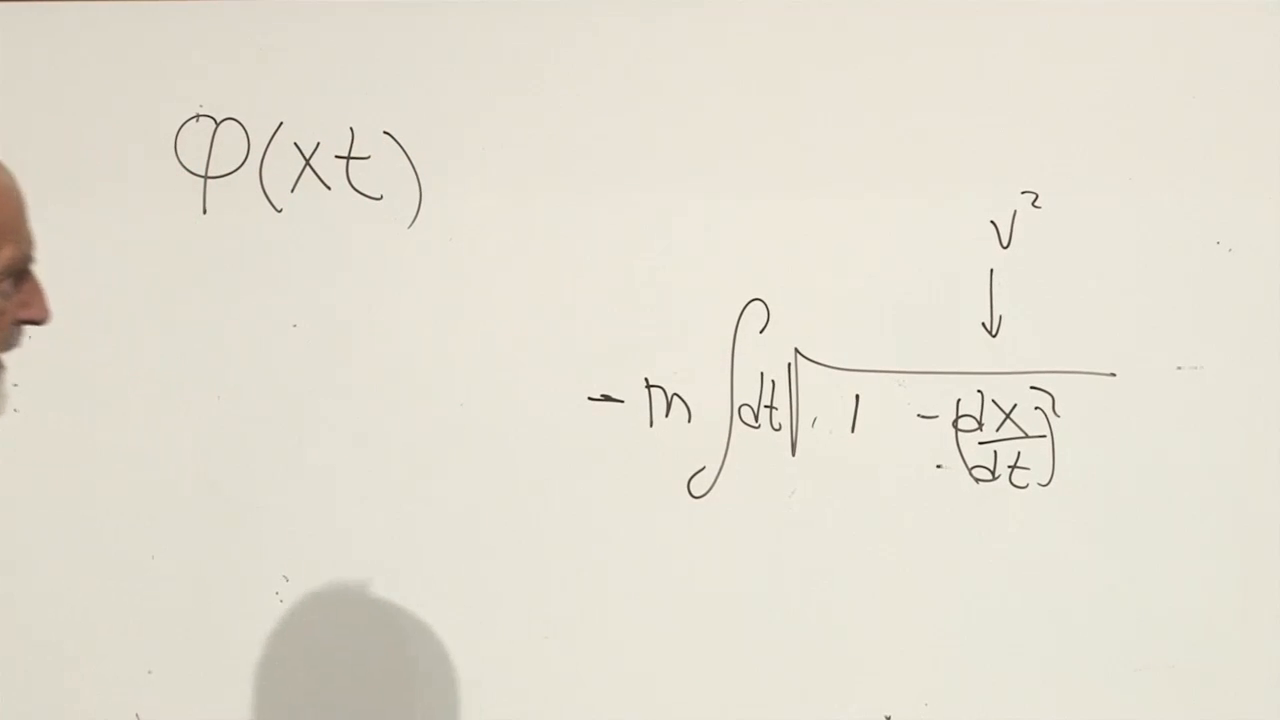
\includegraphics[width=0.90\textwidth]{lecture_04_figure_15.png}
\caption{座標時間のラグランジアンとして書き直された不変な自由粒子作用。}
\lectureframe{01:34:31}
\end{figure}

\subsection{最も単純なスカラー結合}

\(d\tau\)も\(\phi\)もスカラーである。したがって最も単純な線形結合は
\begin{equation}
\boxed{
A
=
\int d\tau\,[-m+\phi(x,t)]
}.
\label{eq:sr4-coupled-action}
\end{equation}
である。この選択は一意ではない。\(\phi\)を任意の関数\(F(\phi)\)で置き換えることもできる。線形項は物理的アイデアを示すのに十分である。

\begin{figure}[htbp]
\centering
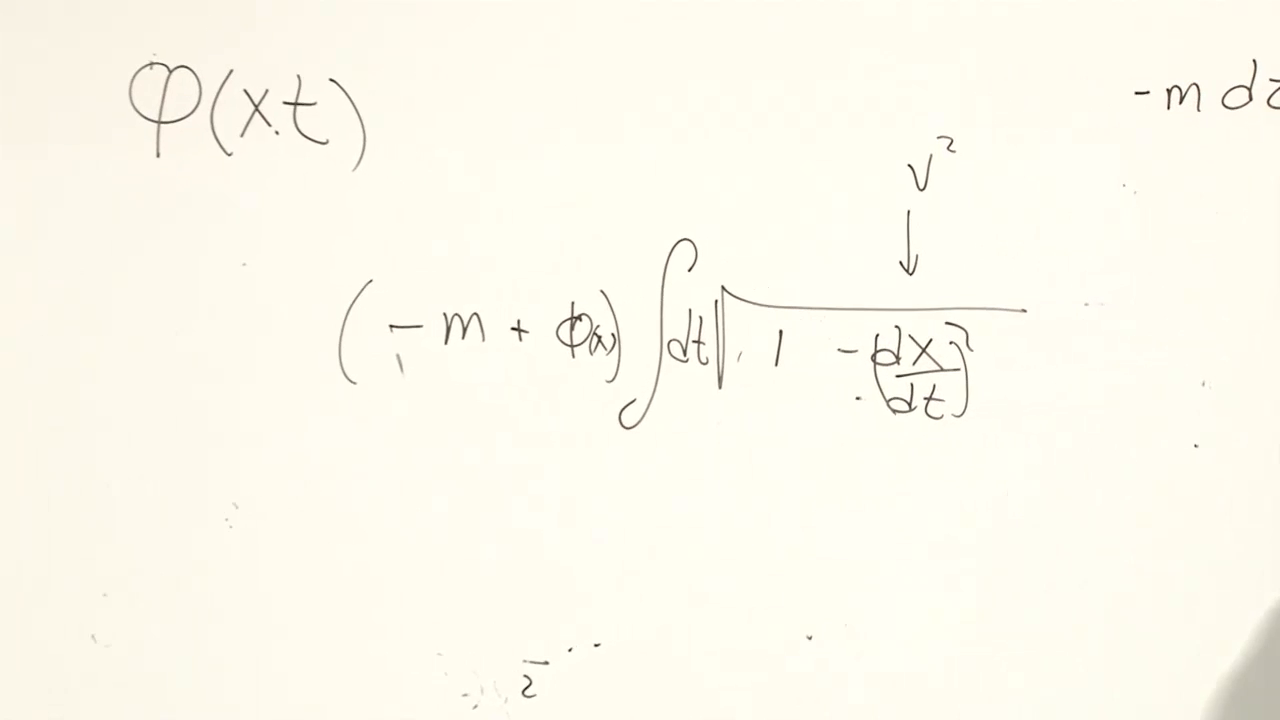
\includegraphics[width=0.90\textwidth]{lecture_04_figure_16.png}
\caption{最も単純なローレンツ不変スカラー結合で補われた自由作用。}
\lectureframe{01:37:21}
\end{figure}

\begin{classroomqa}
\audiencequestion{\(\phi\)は積分の内側にとどまらなければならないのか。}
\lecturerresponse{はい。場は粒子の世界線\(\phi(x(t),t)\)上で評価され、一般に軌道のある点から別の点へと変化する。たとえ背景が陽に時間依存しなくても、\(\phi=\phi(x)\)、粒子が空間を運動するときには依然として時間とともに変化する。経路に沿って一定である場だけが積分の外に出せる。\lecturetimestamp{01:37:47}}
\end{classroomqa}

\begin{classroomqa}
\audiencequestion{\(\phi(x,t)\)の中の\(x\)は粒子の位置を意味するのか。}
\lecturerresponse{はい。それは\(x=x(t)\)、時刻\(t\)における粒子の位置である。作用は、その軌道に沿って与えられた時空場をサンプリングする。\lecturetimestamp{01:38:08}}
\end{classroomqa}

一次元運動に対して、\eqref{eq:sr4-coupled-action}は
\begin{equation}
L
=
-(m-\phi(x,t))\sqrt{1-\dot x^2}.
\label{eq:sr4-coupled-lagrangian}
\end{equation}
を与える。スカラー背景は、ちょうど静止質量が占める場所に現れる。
\begin{equation}
m_{\rm eff}(x,t)=m-\phi(x,t).
\label{eq:sr4-effective-mass}
\end{equation}
もし\(\phi\)がほぼ一定の非零値に落ち着くなら、粒子はその質量がずれたかのように振る舞う。これは単なる古典的玩具模型であり、完全なヒッグス機構ではないが、宣伝されているヒッグス的アイデアの趣を捉えている。すなわち、スカラー背景は質量項として粒子の力学に入り得る。

\subsection{粒子の方程式}

正準運動量は
\begin{equation}
p
=
\frac{\partial L}{\partial\dot x}
=
(m-\phi)
\frac{\dot x}{\sqrt{1-\dot x^2}}.
\label{eq:sr4-coupled-momentum}
\end{equation}

\begin{figure}[htbp]
\centering
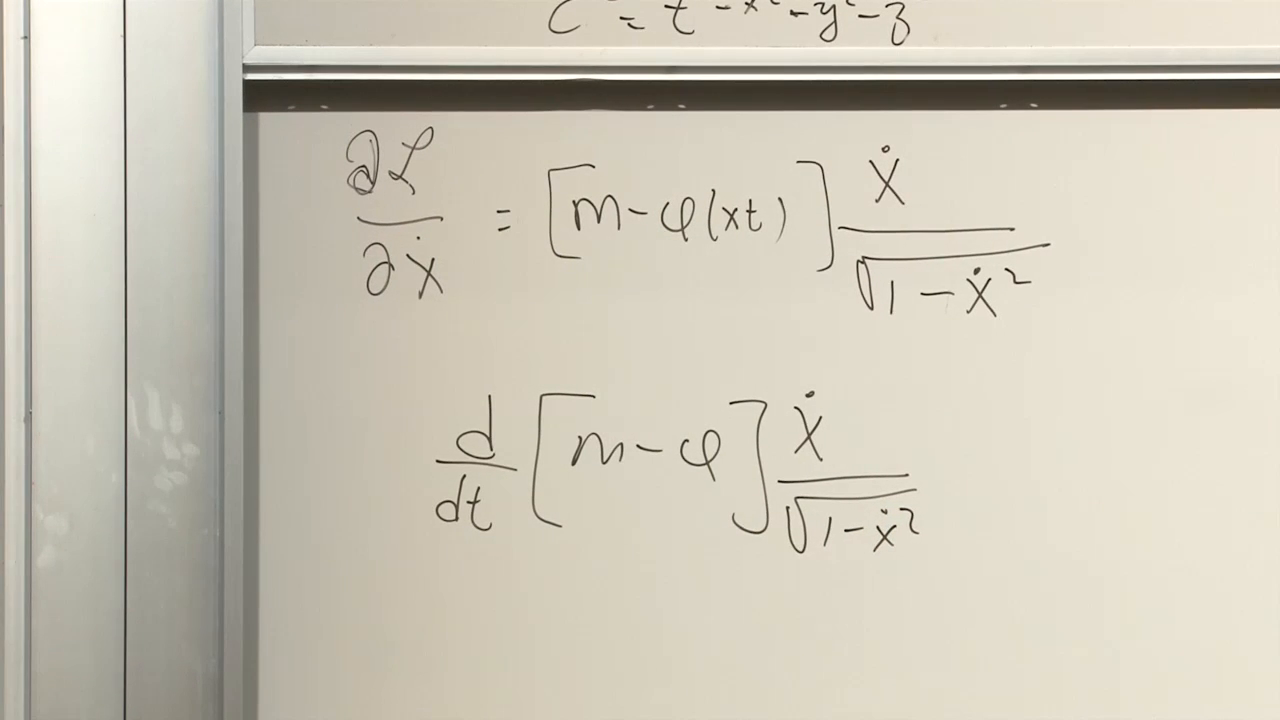
\includegraphics[width=0.90\textwidth]{lecture_04_figure_17.png}
\caption{スカラー背景は、相対論的正準運動量において\(m\)を\(m-\phi(x,t)\)に置き換える。}
\lectureframe{01:43:38}
\end{figure}

ラグランジアンの位置に関する導関数は
\begin{equation}
\frac{\partial L}{\partial x}
=
\frac{\partial\phi}{\partial x}
\sqrt{1-\dot x^2}.
\end{equation}
作用\eqref{eq:sr4-coupled-action}によって符号を固定すると、オイラー--ラグランジュ方程式はしたがって
\begin{equation}
\boxed{
\frac{d}{dt}
\left[
(m-\phi)
\frac{\dot x}{\sqrt{1-\dot x^2}}
\right]
=
\frac{\partial\phi}{\partial x}
\sqrt{1-\dot x^2}
}.
\label{eq:sr4-coupled-eom}
\end{equation}

\begin{figure}[htbp]
\centering
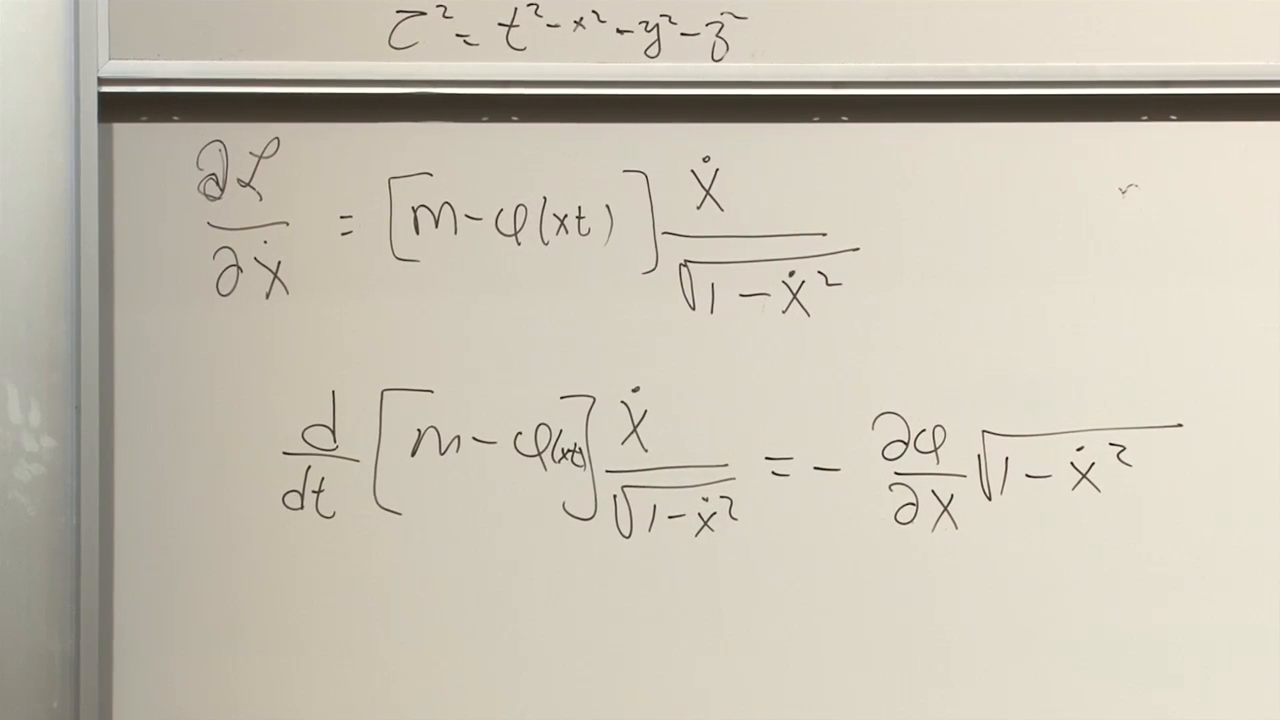
\includegraphics[width=0.90\textwidth]{lecture_04_figure_18.png}
\caption{運動量と背景場の空間導関数から組み立てられる結合方程式。作用が\eqref{eq:sr4-coupled-eom}における最終的な符号を固定する。}
\lectureframe{01:45:24}
\end{figure}

\begin{classroomqa}
\audiencequestion{なぜ\(\partial\phi/\partial x\)は因子\(\sqrt{1-\dot x^2}\)を保つのか。}
\lecturerresponse{\(x\)に関して微分されるのは因子\(\phi(x,t)\)だけだからである。ラグランジアンでは平方根がそれを掛けており、偏微分で\(\dot x\)を固定するとき平方根は位置に依存しないので、平方根は残る。\lecturetimestamp{01:45:50}}
\end{classroomqa}

全時間導関数を展開すると
\begin{align}
&(m-\phi)
\frac{d}{dt}
\left(
\frac{\dot x}{\sqrt{1-\dot x^2}}
\right)
-
\dot\phi\,
\frac{\dot x}{\sqrt{1-\dot x^2}}
\nonumber\\
&\hspace{10em}
=
\frac{\partial\phi}{\partial x}
\sqrt{1-\dot x^2}.
\label{eq:sr4-coupled-expanded}
\end{align}
となる。背景が静的、\(\phi=\phi(x)\)であっても、運動する世界線に沿ったその導関数は零ではない。連鎖律により
\begin{equation}
\boxed{
\dot\phi
=
\frac{d}{dt}\phi(x(t))
=
\frac{\partial\phi}{\partial x}\dot x
}.
\label{eq:sr4-chain-rule}
\end{equation}

\begin{classroomqa}
\audiencequestion{\(\phi\) に明示的な時間依存性がないのなら、なぜ \(\dot\phi\) はゼロではないのか。}
\lecturerresponse{粒子が位置を変えるからである。場は \(x(t)\) でサンプルされるため、その全微分は \(\dot\phi=\phi_x\dot x\) となる。静的な場とは \(\partial\phi/\partial t=0\) を意味するのであって、運動するすべての粒子が一定の場の値を見るという意味ではない。\lecturetimestamp{01:48:10}}
\end{classroomqa}

\begin{figure}[htbp]
\centering
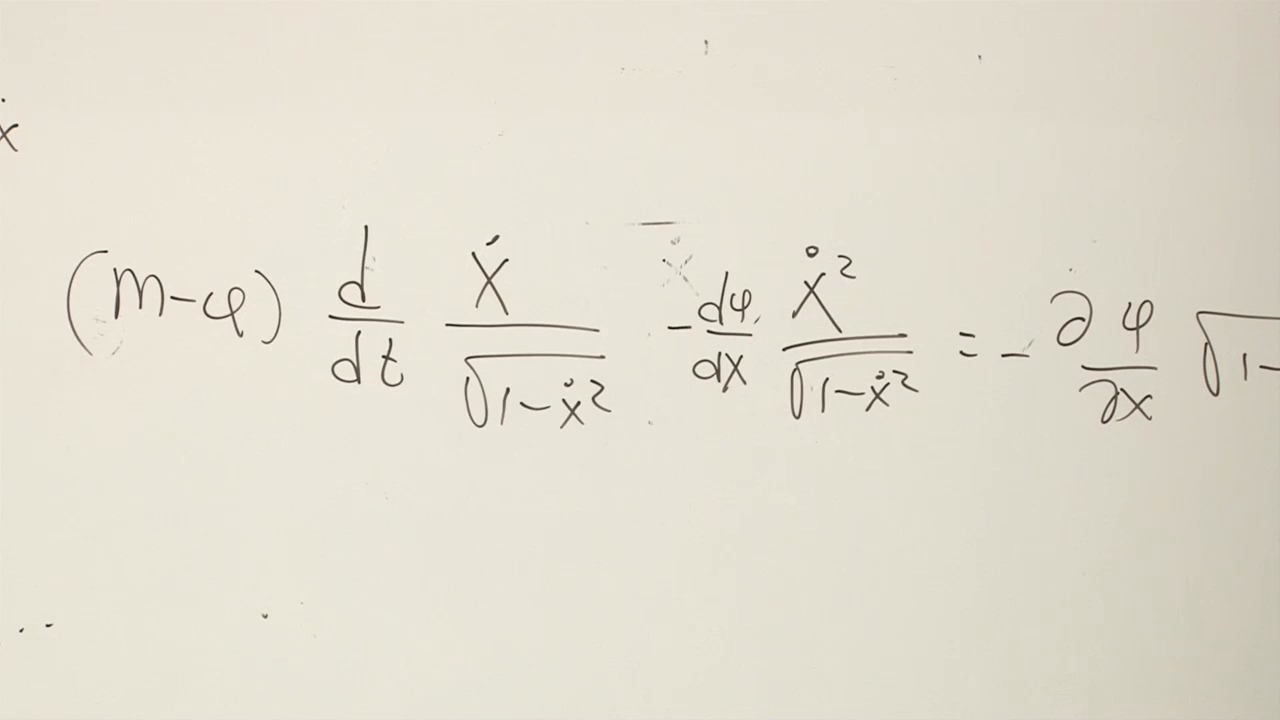
\includegraphics[width=0.90\textwidth]{lecture_04_figure_19.png}
\caption{世界線に沿って連鎖律を用いた後の、連立方程式の後半の展開。}
\lectureframe{01:49:11}
\end{figure}

厳密な表式は特に美しいものではなく、講義もそうでないふりはしない。それでもその低速極限は見慣れたものである。\(\sqrt{1-\dot x^2}\approx1\) であるから、主要な方程式は
\begin{equation}
\frac{d}{dt}\bigl[(m-\phi)\dot x\bigr]
\approx
\frac{\partial\phi}{\partial x}.
\end{equation}
有効質量の変化も摂動的に扱うならば、これは
\begin{equation}
(m-\phi)\ddot x
\approx
\frac{\partial\phi}{\partial x}.
\label{eq:sr4-nonrel-force}
\end{equation}
となる。実際、低速でのラグランジアンは
\begin{equation}
L
\approx
-m+\phi+\frac12(m-\phi)\dot x^2,
\end{equation}
であるから、主要な次数でポテンシャルエネルギーは \(U=-\phi\) であり、力は \(-dU/dx=\partial_x\phi\) である。\(c\) の因子を復元し、このニュートン的なパターンを回復することが、講義を締めくくる演習である。

粒子から場への道筋はこれで完成した。粒子の履歴 \(\phi(t)\) が \(0+1\) 次元の原型を与え、場の履歴 \(\phi(x)\) が作用を時空積分へと昇格させ、場のオイラー--ラグランジュ方程式が波動力学を生み出し、ローレンツスカラーが相対論的な符号構造を選び出し、そして同じ不変な言語によってスカラー背景が粒子に作用を及ぼし返すことが可能になった。